\clearpage

\section{Evaluation}
\label{cp5:evaluation}



The goal of our evaluation is to assist the design of tools that use the explored techniques to help developers in locating text relevant to their task. 
To evaluate and compare the techniques,
we measure what portion of the \acs{DS-android} text identified by human annotators the techniques automatically identify.
We report \textit{precision} and \textit{recall} metrics~\cite{manning2010IR}
focusing on recall since failure to identify text that is relevant to a task (false negatives)
means that a developer will have an incomplete or partial view of the information needed for their task.
Experimental procedures are as follows.



\subsubsection{Baseline}


As done by~\cite{Lin2021} and~\cite{Ye2016}, we use a standard \texttt{VSM} lexical similarity approach as a baseline. Our rationale to use 
lexical similarity as a baseline is based on the fact that 
both our qualitative analysis (\red{Chapter~\ref{aaa}}) and
related work~\cite{Ko2006a, Freund2015} have shown that developers often use keyword-matching as a first search strategy to locate text that might contain information relevant to their tasks.


Analogous to the semantic similarity-based technique (Section~\ref{cp5:approach-w2v}), the baseline technique uses VSM to compute lexical similarity scores 
for all the sentences in an input artifact with regards to an input task and then, it outputs the top-n sentences with highest similarity as the ones likely relevant to an input software task.




\subsubsection{Setup}



We configure each technique to identify a target number of 10 relevant sentences per input task-artifact.
This decision is based on the fact that 
no more than 20\% of the content of any artifact in the corpora is deemed relevant to a task, which, on average, accounts for 8.93 sentences (\red{Chapter~\ref{}}).
Researchers have also used the same target number of 10 sentences when evaluating techniques  (e.g.,~\cite{Xu2017} or~\cite{Lotufo2012}) able to identify relevant text for certain kinds of artifacts
what will also facilitate comparing our results to related work.


\subsubsection{Training Data}


In addition to configuring the techniques output, two of our techniques use part of the  \acs{DS-android} data for fine-tuning purposes (\texttt{BERT}) and to derive sentence-task frame pairs (\texttt{association-pairs}).
We ensure that no data used to evaluate these techniques is also used in their setup by 
splitting the dataset using standard cross-validation techniques.
We split the dataset into 10 folds, each containing 5 tasks used for evaluation purposes. When evaluating a fold, the remaining 45 tasks are used to mine sentence-task frame pairs
and to train BERT. 
For the BERT technique, we further split the training data and use 10\% of it to validate the model~\cite{Chaparro2017, fucci2019, Petrosyan2015}.
We refer to this setup of BERT as \texttt{BERT\textsubscript{DS-android}}.


To study the impacts of training data on BERT, we also train the model in a smaller dataset containing six tasks and a total of 1874 sentences, from which 602 of them were deemed relevant by 20 participants with software development experience (\red{Chapter~\ref{aaa}}). Due to the synthetic nature of the tasks in this dataset, we refer to this 
second configuration as \texttt{BERT\textsubscript{DS-synthetic}}.




\subsubsection{Metrics}


We compute values for \textit{precision} and \textit{recall} metrics using the golden labels available in the \acs{DS-android} corpus and sentences deemed relevant to a task by at least two human annotators.

Precision means identifying only text that is relevant whereas recall means identifying all relevant text.
For a detailed definition of each metric, we refer to the evaluation outcomes detailed in Table~\ref{tbl:type-I-II-errors}, where  columns represent  labels provided by the annotators and rows,
the text identified as relevant or not by a technique.

\medskip
\begin{table}[H]
\centering    
\begin{scriptsize}
\begin{threeparttable}
\begin{tabular}{l|l|l}

\hline

\textbf{}
& \textbf{Relevant}    
& \textbf{Not-relevant} \\

\hline

\textbf{Identified as relevant} & true positive ($TP$) & false positive ($FP$) \\
\hline
\textbf{Identified as Not-relevant} & false negative ($FN$) & true negative ($TN$) \\
\hline

\end{tabular}
\end{threeparttable}
\end{scriptsize}
\caption{Evaluation outcomes}
\label{tbl:type-I-II-errors}
\end{table}

    



\paragraph{\textbf{Precision}}

Precision measures the fraction of the sentences identified that are relevant over the total number of target sentences identified, as shown in Equation~\ref{eq:cp5:precision}.



\begin{equation}
\label{eq:cp5:precision}    
    Precision = \frac{TP}{TP + FP}
\end{equation}



\paragraph{\textbf{Recall}} Recall represents how many of all the annotated sentences are identified by a technique (Equation~\ref{eq:cp5:recall}).


\begin{equation}
\label{eq:cp5:recall}        
    Recall = \frac{TP}{TP + FN}
\end{equation}



\medskip
Ideally, we would aim for a technique with both high precision and recall. In practice, this is often not possible and we must reach a compromise.
Researchers have shown that, in a natural language artifact, developers face more challenges finding information that pertains to their task rather than judging whether the text is relevant or not~\cite{Robillard2015, Maalej2013}. Hence, in a bound number of sentences identified by a technique, we argue that developers can quickly discard what they judge that is not relevant and we aim to identify as much of the relevant text as possible.






% \art{Removed pyramid precision and pyramid recall based on last conversations with Gail}
% \paragraph{\textbf{Pyramid Precision \& Pyramid Recall}} 
% We measure precision and recall considering sentences marked by two or more annotators; this, however ignores the fact that text marked by a single annotator can equally contribute towards task completion~\cite{marques2020}. To address the text identified by a single annotator, we 
% follow evaluation procedures outlined by Lotufo et al.~\cite{Lotufo2012} and we
% also report pyramid precision and pyramid recall. These metrics are similar to the ones defined in 
% Equations~\ref{eq:cp5:precision} and~\ref{eq:cp5:recall} but treat relevant text as the sentences marked by any of the annotators.





\subsection{Results}




Figure~\ref{fig:eval-metrics-results} shows values for F1-score, precision, and recall for each of the techniques that we explore as part of our design space. 



The \texttt{baseline} technique, which uses VSM, achieves precision and recall scores of $0.30$ and $0.33$, respectively. 
Although this result is not surprising, it corroborates results from related literature showing limitations of lexicon-based approaches, and 
it further motivates the need for techniques able to relate the information associated with the solution for a task and the information provided in the software task.


Using word semantics, precision and recall scores increase to $0.48$ and $0.53$ when using \texttt{word2vec}, and to $0.55$ and $0.56$ with \texttt{BERT}.
With regards to BERT, we do not observe significant differences between the \texttt{BERT\textsubscript{DS-synthetic}}
and the \texttt{BERT\textsubscript{DS-android}} configurations suggesting that the model predictions extend to datasets other than the ones used for training.
A potential explanation for that is that 
BERT uses \textit{transfer learning} \red{ref} and thus, the  
large corpora used to train the model before fine-tuning (Section~\ref{cp5:bert}) assists prediction steps even for tasks and artifacts that the model was not trained upon.



\clearpage
\begin{landscape}

\begin{figure}
    \centering
    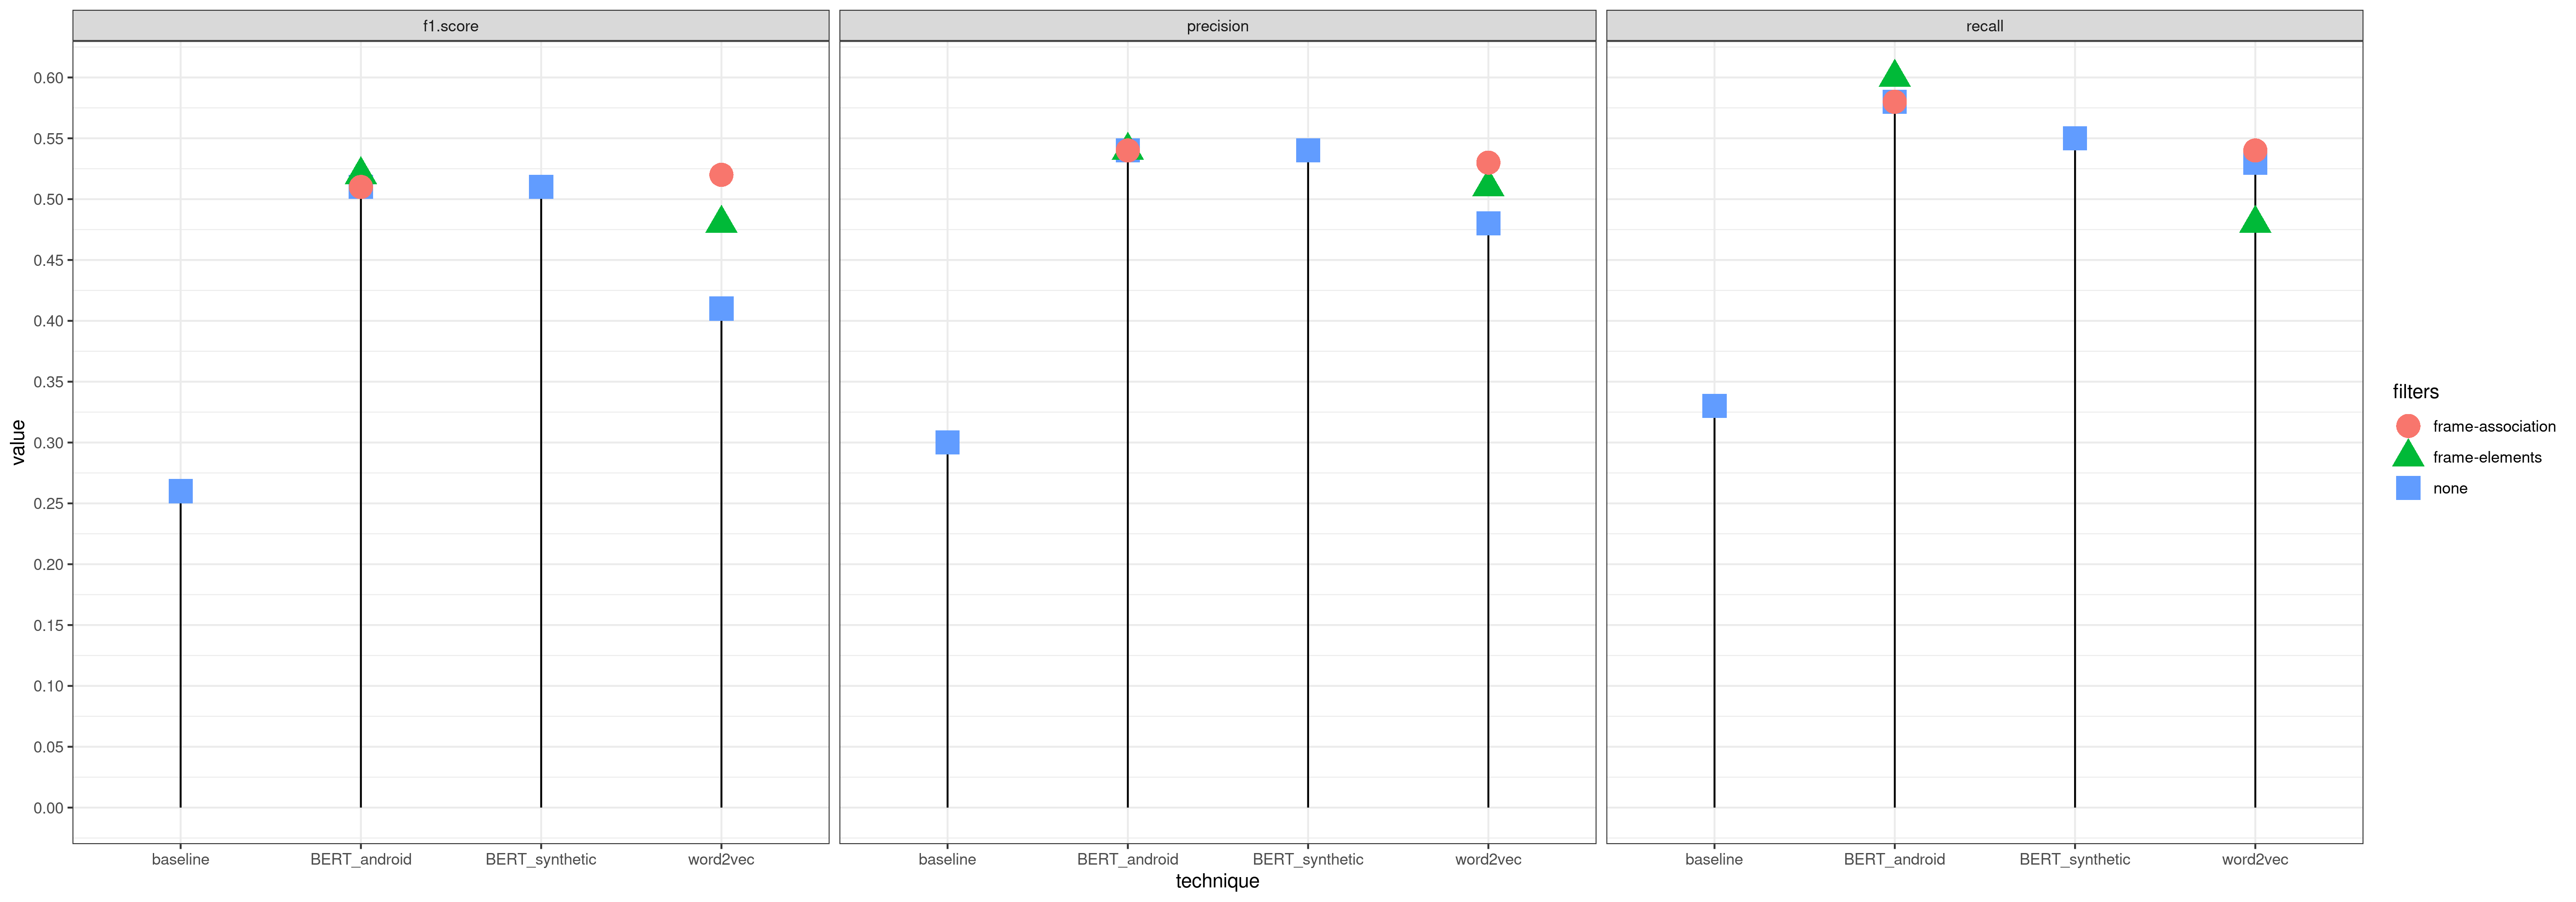
\includegraphics[width=1.8\textwidth]{cp5/results}
    \caption{Evaluation metrics for each techniques \art{image resolution has been finicky. I'll fix it and have the image in-line with the rest of the results}}
    \label{fig:eval-metrics-results}
\end{figure}
\end{landscape}

\clearpage




Figure~\ref{fig:eval-metrics-results} also shows results when applying sentence semantic filters as
 a post-processing step to the
 \texttt{word2vec} and \texttt{BERT} techniques. 
Both filters improve precision and recall values for the \texttt{word2vec} technique, where the \texttt{association-pairs} filter yields 
the highest results ($0.53$ precision and $0.54$ recall). For \texttt{BERT}, there are no noticeable changes to precision, but 
we observe gains on recall. Notably, the \texttt{frame-elements} filter achieves $0.60$ recall for \texttt{BERT\textsubscript{DS-android}}. 



\subsubsection{Pyramid scores}


\art{I did not observe differences between the metrics when considering all the text marked and the text marked only by two annotators. I'll have to further investigate why.}


\subsubsection{Text identified}


To get a better sense of the text identified, we compare the text that each technique identifies as relevant according to the golden data in the \acs{DS-android} corpus, i.e., the text that at least two annotators deemed relevant. For this analysis, 
we use the best configuration for each technique. That is, both the word semantics and sentence semantic filters.



Figure~\ref{fig:text-overlap} shows the overlap between the text identified when the techniques identify up to 10 
sentences per task and artifact.
From 382 unique sentences, the \texttt{baseline} identifies a total of 110 sentences. In comparison, \texttt{word2vec} identifies a total of 213 sentences and \texttt{BERT\textsubscript{DS-android}}, 234 sentences. 
We observe that with the exception of the baseline, the majority of the sentences 
identified are technique-specific. Potential exmplanations for that are related to how each technique 
determines relevance. That is, \texttt{word2vec} uses semantical similarity based on task and artifact's sentences embedding vectors while 
\texttt{BERT} correlates the embeddings of a sentence from a task and from an artifact through the 
\textit{transformers} attention function (Section~\ref{cp5:bert}).




\begin{figure}
    \centering
    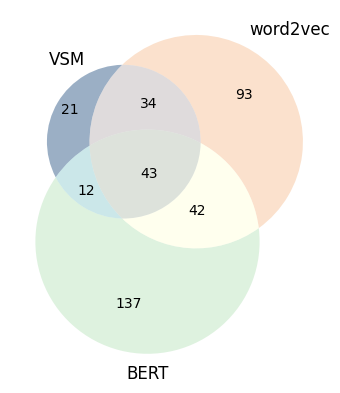
\includegraphics[width=0.4\textwidth]{cp5/results_venn.png}
    \caption{Venn diagram illustrating the overlap between the 382 task-relevant sentences identified across the three techniques}
    \label{fig:text-overlap}
\end{figure}


Analysis of the text identified by each technique suggests that the techniques identify different types of information.


% When interpreting results, it is worth noting that due to the nature of \acs{DS-android} corpus, the fraction of sentences annotated as relevant is considerable small,
% e.g., API documents in the corpus have an average of 109.22 sentences per document while only an average of 9.62 sentences are relevant (Chapter~\ref{ch:android-corpus}). 
% Hence, achieving 
% This means that the data is unbalanced and achieving high accuracy is challenging even when using state-of-the-art techniques.





% \art{Change from tables to plots. Similar to Sarah and Treude~\cite{nadi2020}, show Venn diagram with how many sentences each approach identifies and overlaps between them}




% \begin{table}[H]
\centering    
\begin{scriptsize}
\begin{threeparttable}
\begin{tabular}{llcccc}


\textbf{} & \textbf{Technique} &
\textbf{Precision} & \textbf{Recall} & 
\parbox[c][.7cm][c]{1.5cm}{\centering \textbf{Pyramid precision}} & 
\parbox[c][.7cm][c]{1.5cm}{\centering \textbf{Pyramid recall}} \\


\hline

\multirow{ 2}{*}{\textbf{Baseline}}  & VSM &
0.50 & 0.50 & 
0.50 & 0.50 
\\

& ours &
0.50 & 0.50 & 
0.50 & 0.50 
\\

\hline

\multirow{ 2}{*}{\textbf{API documentation}}  & Kreck &
0.50 & 0.50 & 
0.50 & 0.50 
\\

& ours &
0.50 & 0.50 & 
0.50 & 0.50 
\\

\hline

\multirow{ 2}{*}{\textbf{GitHub issues}} & Hurried &
0.50 & 0.50 & 
0.50 & 0.50 
\\

 & Ours &
0.50 & 0.50 & 
0.50 & 0.50 
\\

\hline

\multirow{ 2}{*}{\textbf{SO answers}} & AnsBot &
0.50 & 0.50 & 
0.50 & 0.50 
\\

 & Ours &
0.50 & 0.50 & 
0.50 & 0.50 
\\

\hline

\end{tabular}
\end{threeparttable}
\end{scriptsize}
\caption{Techniques comparison}
\label{tbl:approach-results-artifacts}
\end{table}








